\documentclass{article}
\usepackage{tikz}
\usepackage{amsmath}
\usepackage[margin=1in]{geometry}

\title{Toolpath Generation for Face Milling of Fused Cuboids}
\author{Generated by M365 Copilot}
\date{\today}

\begin{document}

\maketitle

\section*{Original Prompt}
\textit{You are a software+mechanical engineer tasked with generating a toolpath generation software for solids with some fused cuboids on the same base floor but of different heights and widths and lengths. The top faces boundaries are known. How will you produce the toolpath footprint for face milling the top faces without gouging into vertical walls if they exist. The existence of vertical walls is known. The tool must enter from outside the face.}

\section*{Concept Overview}
Each top face is treated as a machining island at height $Z_i$ with polygon boundary $P_i$. The tool of radius $R$ must remain within a safe configuration space that avoids vertical walls.

\section*{Wall Classification}
For each edge:
\begin{itemize}
    \item If neighbor height $< Z_i$: safe drop-off
    \item If neighbor height $= Z_i$: merge region
    \item If neighbor height $> Z_i$: vertical wall (blocked)
\end{itemize}

\section*{Safe Region Construction}
Define the safe machining region:
\[
S_i = P_i \ominus B_{blocked}
\]
where only blocked edges are offset inward by $R$.

\section*{Entry Strategy}
Entry edges must lie on drop-offs or outer boundaries. Tool enters via linear or arc lead-in from outside.

\section*{Toolpath Strategy}
Zig-zag raster toolpaths are generated inside $S_i$.

\section*{TikZ Illustration}

\begin{center}
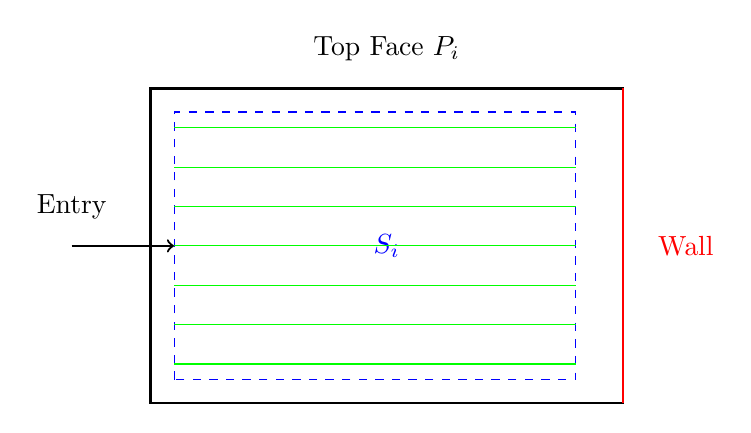
\begin{tikzpicture}[scale=1]

% Original face
\draw[thick] (0,0) rectangle (6,4);
\node at (3,4.5) {Top Face $P_i$};

% Blocked wall edge
\draw[red, thick] (6,0) -- (6,4);
\node[red] at (6.8,2) {Wall};

% Safe region (offset)
\draw[blue, dashed] (0.3,0.3) rectangle (5.4,3.7);
\node[blue] at (3,2) {$S_i$};

% Toolpath lines
\foreach \y in {0.5,1,...,3.5} {
    \draw[green] (0.3,\y) -- (5.4,\y);
}

% Entry arrow
\draw[->, thick] (-1,2) -- (0.3,2);
\node at (-1,2.5) {Entry};

\end{tikzpicture}
\end{center}

\section*{Algorithm Summary}
\begin{verbatim}
for each face (sorted highest to lowest):
    classify edges
    construct safe region
    select valid entry edge
    generate raster paths
    ensure no wall collisions
\end{verbatim}

\section*{Key Insight}
This is a configuration space planning problem where walls are expanded by tool radius and paths are generated for the tool center.

\end{document}
